\documentclass[11pt, a4j, openany, oneside]{jbook}

\usepackage[dvips]{graphicx}
\usepackage{latexsym}
\usepackage{amssymb}
\usepackage[hang,small,bf]{caption}
\usepackage[subrefformat=parens]{subcaption}
\usepackage{SLabMasterThesisStyle}


\year{27} 
\title{独立同期モデルに基づく \\ 初学者の協調プログラミング支援} 
\advisingteacher{酒井 三四郎}
\studentid{7043-0013}
\author{加藤 優哉}
\department{静岡大学大学院情報学研究科 \\ 情報学専攻}


\begin{document}

%表紙出力
\maketitle

\tableofcontents

\chapter{序論}
ICTを活用しながら学習者同士が互いに知識・経験・技能を豊かにし,問題解決の方法を見出し,協調的なプロセスを通して新しい知識を創造する能力が21世紀に必要な能力とされている\cite{griffin2012assessment}.ソフトウェア開発の現場においても,近年では協調的で創造的なソフトウェア開発手法のニーズが高まっている.そのような背景でアジャイルソフトウェア開発手法,特に,知識創造理論\cite{takeuchi1986new}をベースとしたScrum\cite{schwaber2002gile}が注目を集めており,教育現場でもその導入が試みられ始めている\cite{anslow2015experience}.

プログラミング入門教育においても,グループでプログラムを作成する課題が試みられてきた\cite{松浦佐江子2003}\cite{玉田春昭}.しかしながら,実際の現場では,初学者がグループプログラミングを通して,協調的な創造活動を行うことは困難である.我々の現場の観察では,典型例として,(1)プログラムの大半をグループで最も得意な学生が記述してしまい,その他のメンバはプログラムを書かない,(2)グループメンバが完全にタスクを分割して作業をしてしまう(例えば,複数の小規模なサブゲームから成るゲームをそれぞれ完全に独立して制作する)などという問題が観察される(\ref{State}節にて詳説).

初学者がグループプログラミングで使用するツールにも問題がある.理想としては,構成管理ツール(e.g. subversion, git,mercurial)を駆使してプロジェクトを進めることが望ましい.しかしながら,プロフェッショナル向けにデザインされているためツールの操作や概念が複雑で,プログラミング入門講義の学習者が使用するのは困難である.プログラミング入門教育で学習者が集中すべきなのはアルゴリズム構築であり,このようなツールの利用方法に関して学ぶ時間は用意されていない.

本研究では,これらの問題を解決するために,初学者向けの協調プログラミング支援システム「CheCoPro」を提案する.初学者が容易に利用でき,かつ能力差があるグループでも,個々人が並行的に作業し,貢献できる構成管理ツールのモデルを考案し,実際の授業で試行した.システムの利用ログを利用することで初学者のグループプログラミングにおけるインタラクションを視覚化することで,インタラクションの実態解明と合わせてツールの評価を行った.

本論文は全\ref{CC}章からなる.プログラミング教育における「協調プログラミング」の定義を\ref{Def}章で行う.\ref{RW}章で,グループプログラミングを支援する既存ツールのレビューを行う.\ref{Model}章では,初学者に協調プログラミングを支援するツールのモデル「独立同期モデル」を提案する.\ref{CH}章では,\ref{Model}章で提案したモデルに基づいて設計・実装したシステムを説明する.\ref{EM}章で評価実験の方法,\ref{RS}章ではその結果を報告する.\ref{DC}章で考察を行う.\ref{CC}章はまとめである.
	
\chapter{協調プログラミング}\label{Def}


%----------2.1--------
\section{ソフトウェア開発における協調作業のモデル}

プログラミング/ソフトウェア開発における協調作業のモデルは,ソフトウェア工学の分野で30年以上にわたって議論され続けてきた.中でも,ウォータフォールモデルとアジャイルモデルの2つのモデルが主要である.ウォータフォールモデルは要件定義,デザイン,実装,テストのようなプロセスを完全に分担するモデルであり,30年以上にわたって最も有力なモデルであった.対照的にここ10年では,アジャイルモデルの人気が上昇している.アジャイルモデルは,柔軟で創造的なソフトウェア開発が要求される産業的な開発においても,状況変化や新しいソフトウェア開発の進化に適している.特に,Scrum\cite{schwaber2002gile}はソフトウェア開発方法論の中で現在最も人気のある方法である.Scrumは知識創造理論\cite{takeuchi1986new}がベースとなっている.従って,ウォーターフォールモデルとは正反対の協調作業が行われる.例えば,プロジェクトマネージャによる管理に代わって,自己組織化プロセスが推奨されることが挙げられる.Scrumでは,役割分担をするのではなく,作業を共有し暗黙知を共有することが推奨される.

現在,プロフェッショナルと教育現場の双方で,協調プログラミングでの各モデルの利点が議論されている.我々のモデルは主にアジャイルモデルと知識創造理論に基づいている.近年,参加者間の論理的なインタラクションと役割やリーダの頻繁な変更が,オープンソースソフトウェア開発コミュニティのような創造的なコミュニティで観察された\cite{kidane2007correlating}.教育現場でも同様の現象が観察されている\cite{knutas2013communication}.その他の研究においても,協調プログラミングにおいて学習者間のインタラクションの重要性が主張されている.平井らは,プログラミング学習について参加者が意見交換,競合,交渉,合意形成等を繰り返し,グループの合意としての成果を出すことを協調プログラミング学習と定義している\cite{平井佑樹2012}.

ソフトウェア開発の現場の観点から,ペアプログラミングとその利点について議論され続けている.ペアプログラミングはアジャイルモデルの前身であるeXtreme Programming(XP)\cite{beck2000extreme}の12のベストプラクティスのうちの1つである.Cockburnらは協調プログラミングのモデルとして,ペアプログラミングを拡張した「side by sideプログラミング」を提案した\cite{cockburn2000costs}.Goldmanらは,リアルタイム共同コーディング環境の使い方として,(1)授業でのプログラミング,(2)テスト駆動ペアプログラミング,(3)マイクロアウトソーシング,の3つを提案した\cite{goldman2011real}.しかし,協調プログラミングの部分的な成功にとどまり,結果は,教育での小規模のチームにおいて協調学習の促進に成功したのみであった.


%----------2.2--------
\section{入門環境における協調プログラミングの現状}\label{State}

我々は,プログラミング入門授業の場で,最終課題として1チーム2, 3名から構成されるグループプログラミングを実施してきた.現状調査のために,2013年度の授業でアンケートと観察による協調プログラミングの調査を行った.約100名の受講者に対するアンケートを行い,70件の有効回答を得た.

%半分以上を%にかえて,比較できるようにする.このままだと,その他のメンバも結構いけてる雰囲気がしてしまう.
我々が最も注目したのは,グループメンバ間の能力差についてである.まず,各グループのメンバについて次の2つの役割に分類した.

\begin{description}
	\item[ドライバ] グループ内で,コーディングにおいてプロジェクトに最も主体的に参加しているメンバ
	\item[フォロワ] ドライバ以外のメンバ
\end{description}

ドライバとフォロワの実際の記述量に関するアンケート\footnote{学習者の主観による}の結果,グループ内で最もプログラミングに対する得意意識が高い学習者は,成果物のソースコードの記述量の平均が67\%であることことがわかった.その他のメンバのソースコード記述量は,平均28\%であり,全く記述していない学習者も存在した.

%入門環境における協調プログラミングにおいて以上のような現象が発生しており,各グループのメンバについて次の2群に分類可能であることがわかった.我々は,それぞれをドライバとフォロワと名付けた.

観察結果から,2つの典型的な問題があることもわかった.

1つ目の問題は,個々の能力に見合わない不適切な役割分担である.我々は,プロジェクトに費やす時間やソースコードの記述量が,グループメンバ同士で等しくなるように課題に取り掛かることは意図していない.しかし,学習者は各グループメンバの責任を平等にするために,作業量が等しくなるように無理に役割分担を行うことがある.

2つ目の問題は,プロジェクトが完全に独立した作業から成ることである.例えば3人グループのプロジェクトにおいて,メンバそれぞれが1つのミニゲームを作り,それをまとめて3つのミニゲームから成るソフトウェアを成果物とするグループがある.この作品は,単に3つのプロジェクトを個別に開発したのみであり,協調的な作業とは言えない.
%「加算的」はこの場合の意図したいことを意味しない.


%----------2.3--------
\section{協調プログラミングの定義}

%超高度,文献でサポート出来ると良い
%「創発」,「協調学習」,「協調」の定義とかね.
我々が目指す協調プログラミングは,\ref{State}節で述べた2つの問題を解決し,グループメンバ同士のインタラクションによって,創発的に創造的な成果を生み出すような活動が行われるものである.本研究における協調プログラミングは,以下の2つの要件を満たすものとする.


\begin{description}
	\item[collective contribution] 能力が一律ではないグループのメンバ個々人が実力に見合った貢献ができていること.
	\item[productive interaction] グループメンバのインタラクションによって,各メンバの知識・能力が相乗的にプロジェクトに反映されていること.
\end{description}


collective contributionの達成は,フォロワの遠慮を取り除くことで可能であると考えられる.フォロワの遠慮は,ドライバに最新のプロジェクトを送信するように要求する時や,ドライバのソースコードを編集する時に発生することがある.フォロワの遠慮を取り除くことで,フォロワが積極的にプロジェクトに参加可能となる.結果,能力に見合った貢献が可能となると考えられる.

productive interactionの達成は,フォロワの貢献度合いに依存するものと考えられる.ドライバよりもプログラミングが苦手とされるフォロワの貢献は,ドライバや他のフォロワとのインタラクションから発生すると考えられる.

\chapter{先行研究}\label{RW}

CSCW(Computer Supported Cooperative Work)やCSCL(Computer Supported Collaborative Learning)という分野で,グループでのプログラミングを支援するために多くのツールが提案されてきた.

Collabodeは教育目的でデザインされた最新のツールである \cite{goldman2011real}.Collabodeは,複数の学生が同時にソースコードを編集可能なリアルタイム同期環境である.Vandeventerらも同様なツールを提案している \cite{vandeventer2012codewave}.技術的には,一般的な文書のための同時編集環境のライブラリであるEtherPadを基にしている.このライブラリはGoogle Docにも用いられている.同様なツールとしてはSarosがある \cite{salinger2010saros}.SarosはEcipseのプラグインとして実装されている.このツールは指定したメンバの視野(スクロールやファイル選択)を追従する機能が実装されている.Salingerらはグループメンバの意識共有を支援し,コードレビューや遠隔でのペア・パーティプログラミングの際に有用であると主張している.

しかし,リアルタイム同期モデルは営利的なソフトウェア開発やオープンソースプロジェクトのようなプロフェッショナル向けの協調プログラミングではほとんど使われていない.開発現場では,プロフェッショナルはCVSやsubversion,GitのようなSCM(Source Configuration Management)支援ツールを30年以上使っている.現在では,Git / Githubがオープンソースコミュニティでのスタンダードなツールである.これらのツールは最新のツールにも関わらず,単にブランチ&マージモデルを支援しているだけであり,リアルタイムシェアリングはできない.

現在,教育目的でのリアルタイム同期モデルとブランチ&マージモデルの利点は明らかになっていない.一般的な文書の記述において,リアルタイム同期環境の利点の解明に取り組んでいる研究は存在する \cite{brodahl2011collaborative}\cite{zhou2012google}.Andr\'eらは,規則的な作業においては利点を有するが,複雑な創造的なタスクを同時に取り掛かることには不利であると主張している \cite{andre2014effects}.一方で,プログラミングの入門教育において,SCMを取り入れて成功したという報告はない.我々は,リアルタイム同期モデルでは学生の編集が直接的にグループの作品に影響を与えてしまうことを問題と考えている.その他の問題として,時間を共有する必要があるため授業時間外の共同作業を促進できない点が挙げられる \cite{zhou2012google}.対照的に,ブランチ&マージモデルは,遠慮や時間を共有することがないという点で融通がきく.このモデルの問題は,モデルの概念やツールの操作を学ぶために大きな認知的負荷を要することである.特に,一度コンフリクトが発生するとプロフェッショナルでさえも解決に手間がかかるほどである.

以上のように,コミュニケーションや遠隔でのペアプログラミング支援,プロフェッショナル向けのSCMが提案されている.しかし,初学者が使用可能かつ「協調プログラミング」を支援可能なシステムは開発されていない.

\chapter{独立同期モデルの提案}\label{Model}

\begin{figure}[tb]
\begin{tabular}{lr}
	\begin{minipage}[t]{0.5\hsize}
		\centering
		\includegraphics[keepaspectratio, scale=0.225]{img/SCMModel.eps}
		\subcaption{SCMモデル}\label{fig:SCMModel}
	\end{minipage}

	\begin{minipage}[t]{0.5\hsize}
		\centering
		\includegraphics[keepaspectratio, scale=0.225]{img/RAEModel.eps}
		\subcaption{リアルタイム共有モデル}\label{fig:RAEModel}
	\end{minipage}
	\\
	\\
	\multicolumn{2}{c}{
	\begin{minipage}[b]{1\hsize}
		\centering
		\includegraphics[keepaspectratio, scale=0.225]{img/IARModel.eps}
		\subcaption{独立同期モデル}\label{fig:IARModel}
	\end{minipage}
	}
	
	\end{tabular}
	\caption{協調プログラミング支援システムのモデル比較}
	\label{fig:Models}

\end{figure}

本章では,既存の分散型構成管理システムをモデル化し,その特徴を述べた後,本研究で初学者が利用出来るように考案したモデルを提示する.既存のモデルを2つにモデル化し(a) SCMモデル,(b) リアルタイム共有モデルとし,我々が考案した(c) 独立同期モデルとともに,\figref{fig:Models}に示す.


%----------4.1---------
\section{(a) SCMモデル}

SCMモデルは,gitのようなソースコードの変更履歴を記録・追跡するための分散型構成管理ツールのモデルである.SCMモデルを\figref{fig:Models}(a)に示す.図のフォルダアイコンはプロジェクトフォルダを表す.実線矢印は同期,破線矢印は取り込みを表す(他2つのモデルも同様である).SCMモデルは以下の特徴を持つ.

\begin{enumerate}
	\item 1人で複数のブランチを管理することができる.
	\item push・fetch操作により最新バージョンを共有する.
	\item 取り込みはmarge(差分取込)を用いる.
\end{enumerate}

SCMモデルには2つの問題点がある.

1つ目は,pushやfetch,mergeといった様々な専門用語の概念や操作方法が初心者にとって複雑な点である.プログラミング入門教育においては,他に重要な学習項目が多数あるため,このような不必要な学習負荷は避けるべきである.

2つ目は,ドライバが最新のプロジェクトをpushしなければ,フォロワがドライバの最新のプロジェクトを入手することができない点である.このような状況の際に,フォロワはドライバに最新のプロジェクトをpushするように要求する必要がある.しかし,フォロワはドライバの作業を阻害してしまうことを恐れて要求できないことがある.


%----------4.2---------
\section{(b) リアルタイム共有モデル}

リアルタイム共有モデルは,Sarosのようなリアルタイムにファイルを同期し,多人数で同時に同一ファイルへの書き込みが可能なツールのモデルである.リアルタイム共有モデルを\figref{fig:Models}(b)に示す.リアルタイム共有モデルは以下の特徴を持つ.

\begin{enumerate}
	\item グループ内の全てのメンバが1つのプロジェクトを共有する.
	\item 共有されたプロジェクトはリアルタイムに更新・表示される.
	\item 全てのメンバが共有されたプロジェクトを同時に編集できる.
\end{enumerate}

リアルタイム共有モデルの問題点は,ソースコードを編集することがフォロワにとって困難である点である.このモデルは,個人の編集がグループで共有しているファイルに直接変更を加えるため,ドライバが制作したプログラムをフォロワが壊してしまうということが起こり得る.従って,ソースコードの編集には注意が必要となり,フォロワがプロジェクトに参加しづらい.


%----------4.3---------
\section{(c) 独立同期モデル}

独立同期モデルは,プログラミング初心者の協調プログラミングを促進するために,我々が提案するモデルである.独立同期モデルを\figref{fig:Models}(c)に示す.独立同期モデルは以下の特長を持つ.

\begin{enumerate}
	\item 独立した個々のブランチを管理する.
	\item グループメンバの最新バージョンをリアルタイムに閲覧できる.
	\item グループメンバのソースコードを単純操作で取り込むことができる.
\end{enumerate}

特長(1)によって,複数のブランチを管理するようなSCMモデルの複雑さが解消される.グループのプロジェクトに直接干渉してしまうというリアルタイム共有モデルの問題点も解消されると考えられる.この特徴によって,フォロワはドライバのプロジェクトを直接編集してしまうような心配がなくなり,積極的にプロジェクトに貢献ができるようになると考えられる.

特長(2)はリアルタイム共有モデルの利点を採用し,SCMモデルの問題点を解決している.グループメンバに最新バージョンのpush要求を行う必要がなく,他のメンバの作業を中断する心配を解消することができる.この特長によって,フォロワはドライバへのファイル送信要求をする必要がなくなる.結果,フォロワの遠慮が減少することが予想できる.

特長(3)によって,ツールの操作方法などを学ぶ学習負荷を解消することができる.取り込みが容易であれば取り込み回数も増え,他のメンバのソースコードの閲覧・編集が行われる可能性がある.これは,productive interactionの手助けになると考えられる.

\chapter{CheCoPro}\label{CH}

独立同期モデルに基づいて,協調プログラミング支援システムCheCoPro(Cheerful Collaborative Programming)を設計・実装した.CheCoProはクライアント・サーバ方式を利用したシステムである.サーバは新規開発し,クライアントは,我々が開発し,授業で利用しているプログラミング初学者用の開発環境上に組み込む形で実装した.開発言語はクライアント・サーバともにJava(version 1.8)である.

%----------5.1--------
\section{インタフェース}

\begin{figure}[tb]
	\begin{center}
		\includegraphics[width=\linewidth]{img/Interface.eps}
		\caption{CheCoProによるファイル共有の概略図}
		\label{fig:ev}
	\end{center}
\end{figure}


\begin{figure}[tb]
	\begin{center}
		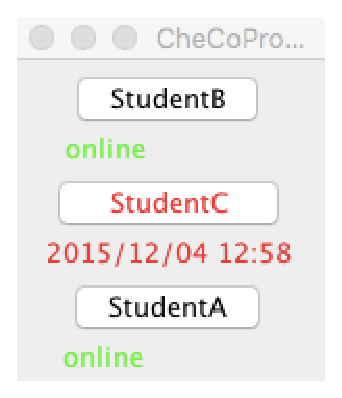
\includegraphics[scale = 0.5]{img/member.eps}
		\caption{メンバセレクタ}
		\label{fig:ms}
	\end{center}
\end{figure}

\begin{figure}[tb]
	\begin{center}
		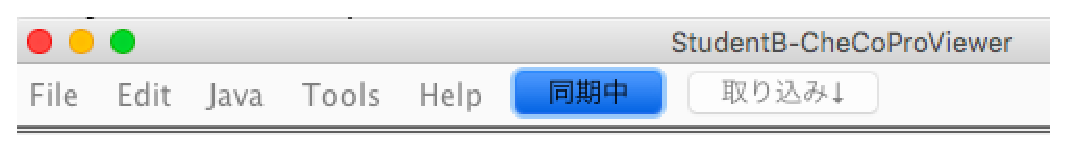
\includegraphics[width=\linewidth]{img/menu.eps}
		\caption{メニューバー}
		\label{fig:mb}
	\end{center}
\end{figure}

CheCoProによるファイル共有の概略図を\figref{fig:ev}に示す.エディタは自身のプログラムを記述するためのウィンドウである.ビューアはメンバのプロジェクトを閲覧するためのウィンドウである.ビューアは,メンバセレクタ(\figref{fig:ms})上のメンバのIDが表示されたボタンをクリックすることで開く.メンバセレクタ上に黒字で表示されているメンバはオンラインであり,赤字で表示されているメンバはオフラインである.ビューアのメニューバー(\figref{fig:mb})から同期状態にするか否かや,全部取込操作を行うことができる.

以下,同期機能と取り込み機能の詳細を説明する.


%----------5.2--------
\section{同期機能}

同期機能は,グループメンバの最新のプロジェクトをリアルタイムに受け取り,それを観察できる機能である.ユーザが自身のエディタ上でソースコードの編集を行うと,その様子が他のメンバのビューアにリアルタイムに反映される.ビューアでは,編集を観察するだけでなく,プログラムを実行して動作を確認することも可能である.

ビューアではソースコードの編集ができない.つまり,他のメンバのソースコードを直接変更できない仕様である.これは独立同期モデルに基づいた設計である.他のメンバのソースコードを編集したい場合,編集したいソースコードを取り込み自分の変更を加え,他のメンバが取り込むという手順が必要である.

ビューアのメニューバーから同期/非同期の切り替えを可能とした理由は,ビューアからメンバのプログラムを実行可能にするためである.同期中はメンバの変更をリアルタイムに受け取るため,プログラムをコンパイルし,実行することができない.非同期中に切り替え,コンパイルエラーが発生するような状態なら自身で修正をして実行することができる.


%----------5.3--------
\section{取り込み機能}

取り込み機能とは,単純な操作でグループメンバのファイルを取り込むことができる機能である.CheCoProでは,2種類の単純な取り込み方法を提供している.1つは全部取込であり,もう1つは部分取込である.

全部取込は,1人のグループメンバが持っているファイルを1度に全て取り込むというものである.全部取込を行う際に,プロジェクトの中のファイルを全て取り込むか,ソースファイル(Javaファイル)を取り込むか,素材ファイル(画像や音楽ファイル)を取り込むかを選択することが可能である.取り込む際に,自身のプロジェクトに同名ファイルが存在する場合は上書きされる.

部分取込は,コピー\&ペーストによる手動の取り込み方法である.ユーザはビューアから取り込みたい部分をコピーし,エディタ上に貼り付けるという単純操作でソースコードを取り込むことができる.

以上の2点の操作には特別な知識は必要としないため,初心者でも容易に行うことができると考えられる.

\chapter{実験方法}\label{EM}

CheCoProの協調プログラミング支援効果の検証を目的に実験を行った.初学者の協調プログラミングにおけるインタラクションのパターンの抽出と,アンケートによる協調プログラミングの意識調査を行った.

%----------6.1--------
\section{学習環境と課題内容}

2014年度秋学期に開講された静岡大学のプログラミング入門講義において実験を行った.プログラミング入門講義は,週2コマの必修の授業である.受講者は,情報学部情報社会学科(文科系)1年生である.実験を行うまでに,受講者はオブジェクト指向の概念を除くJavaの基礎的な学習に4ヶ月間取り組んでいる.協調プログラミングに取り組むことは未経験である.


\begin{table}[tb] 
\caption{課題内容} 
\label{tab:final}
\hbox to\hsize{\hfil
\begin{tabular}{l|ll}\hline\hline
課題		& Javaを使ったGUI作品制作 \\
期間		& 2週間 \\
グループ人数 	& 1〜3名 \\
構成メンバ	& 受講生同士で任意に決定 \\\hline
\end{tabular}\hfil}
\end{table}


実験は,当該講義の最終課題として行った.最終課題の要項を\tabref{tab:final}に示す.最終課題の内容は,Javaを用いたGUI作品の制作である.課題に取り組む期間は2週間である.グループは上限3名であり,メンバは受講者が任意で決めたものである.


%----------6.2--------
\section{システムの導入と利用群,非利用群のグループ分け}

まず,最終課題にエントリした全44組(104名)から,1人グループ8組を除いた36組(96名)を分析対象とした.

CheCoProの導入方法と機能に関する説明を行った上で,CheCoProを利用するかどうかは任意とし,最終的にそのグループの利用状況で利用群と非利用群を分けた.その結果を\tabref{tab:record}に示す.
利用群は15組(3人グループ8組,2人グループ7組),非利用群は21組(3人グループ16組,2人グループ5組)であった.

\begin{table}[tb] 
\caption{グループの内訳と成績} 
\label{tab:record}
\hbox to\hsize{\hfil
\begin{tabular}{c|cc}\hline\hline
				& 利用群 	& 非利用群 \\\hline
組数(割合)		& 15組(41.7\%)	& 21組(58.3\%)\\
成績の平均\footnotemark[2] 	& 51.2 (sd=7.38) 	& 49.4 (sd=8.99) \\\hline
\end{tabular}\hfil}
\end{table}


\footnotetext[2]{この時点までに取得できる成績の最高点は73である} 

この時,CheCoProの導入方法と機能に関する説明は,被験者全員に対して行った(約10分)その後,全グループに対して,CheCoProがすぐに使えるよう初期設定を行った.このようにして,初期設定の煩わしさを理由としてCheCoPro非利用を学習者が選択することを避けた.

この方式での利用,非利用群の分離は,学習者が学習の状況を考えて環境を学習者自身が選択できる反面,利用群と非利用群にプログラミングの能力差が出る可能性がある.そこで,各群のプログラミング能力が概ね等質であることを調べるために,各群の成績の差を調べた.\tabref{tab:record}に示された成績は最終課題に入る前までの講義の成績であり,課題の提出状況と提出物の内容から,講義担当者と著者を含むティーチングアシスタントによって確定したものである.利用群の平均は51.2(sd=7.38),非利用群の平均は49.4(sd=8.99)であった.t検定(以下,断りのない限りWelchの法による)を行った結果,平均の差は有意でなかった(両側検定:t(89.0)=1.10,n.s.).以上より,両群のプログラミング能力について同等であることを確認した.

%----------6.3--------
\section{分析方法}

%----------6.3.1------
\subsection{アンケート}

協調プログラミングに対するフォロワの意識調査から,独立同期モデルの有効性を検証するために,アンケート結果の分析を行った.

アンケート項目の中で,協調プログラミングの達成に重要と考えられる「遠慮」と「貢献」について尋ねたアンケート結果に関して分析を行った.協調プログラミング中の遠慮と貢献の度合いを,「強くそう思う」「そう思う」「そう思わない」「強くそう思わない」の4段階のリッカート尺度を用いて自己評価を行うアンケート項目である.

フォロワの意識の変化が協調プログラミングの成功に繋がると考えられるため,成績の順位を用いて,グループ内のでの順位が1位の者以外をフォロワとして抽出した.ドライバはコーディングにおいてプロジェクトに最も主体的に参加しているメンバと定義したとおり,プロジェクトに積極的に貢献していることが前提である.しかし,フォロワの貢献度合いに関してはグループごとによって異なっていた.


%----------6.3.2------
\subsection{インタラクションパターン}


\begin{figure}[tb]
	\begin{center}
		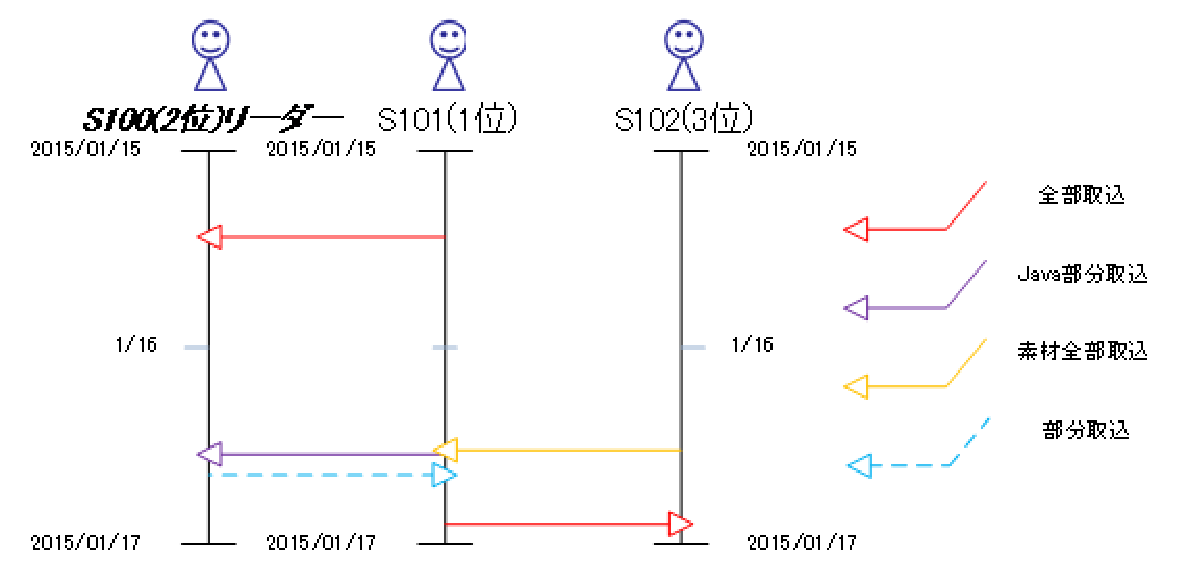
\includegraphics[scale=0.4]{img/flowSample.eps}
		\caption{インタラクション図(例)}
		\label{fig:flowSample}
	\end{center}
\end{figure}


プログラミング初学者の協調プログラミングの実態解明を目的に,インタラクション図の作成と質的分析による評価を行った.

インタラクション図とは,グループメンバ同士の取り込みのやりとりを時系列に表した図である.インタラクション図の例を\figref{fig:flowSample}に示す.縦軸は時間を表す.それぞれの軸の上に記述されている番号はメンバのIDであり,括弧内の数字はグループ内での成績の順位を表す.グループのリーダ\footnotemark[3] は左端に配置し,その他のメンバは左から成績の高い順に配置した.各矢印は取り込みを表し,矢印先のメンバが矢印元のメンバのソースコード等を取り込んだことを表す.

\footnotetext[3]{グループのリーダはグループメンバ同士で任意に決めたものである}

インタラクション図は利用群全15グループに対して作成した.インタラクション図に対する質的な分析から典型的なインタラクションのパターンを抽出することを試みた.

インタラクション図は,ファイルやソースコードの取り込みを表す図である.したがって,被験者がどのような意図で取り込みを行ったのかは把握できない.被験者の行動の意図については,取り込みを行った日時,頻度,ファイルの種類等,インタラクション図の文脈からの推測となる.しかし,推測は被験者に対するインタビューの経験2例から概ね正確であることがわかっている\cite{加藤優哉2014}.


%----------6.3.3------
\subsection{インタラクションと成績}

グループ内のプログラミング能力の差とインタラクションの関係性を調査するために,同講義の成績を用いて分析を行った.本分析では,collective contributionにおけるCheCoProの有効性の検証を試みた.

成績がドライバに近いフォロワはソースコードの提供による貢献をし,ドライバよりも著しく成績が低いフォロワはテストによる貢献にとどまると考えられる.従って,フォロワについて,ソースコードの提供による貢献かテストによる貢献のいずれか一方での貢献に偏っていることが顕著に現れているグループのインタラクション図を抽出した.抽出したグループに関して各メンバの成績と照らし合わせることによって分析を進めた.

\chapter{実験結果}\label{RS}


%----------7.1--------
\section{アンケート結果}


\begin{figure}[tb]
	\begin{center}
		\includegraphics[scale=0.5]{img/diffidence.eps}
		\caption{協調プログラミングにおけるフォロワの遠慮}
		\label{fig:Diffidence}
	\end{center}
\end{figure}

%\samepage

\begin{figure}[tb]
	\begin{center}
		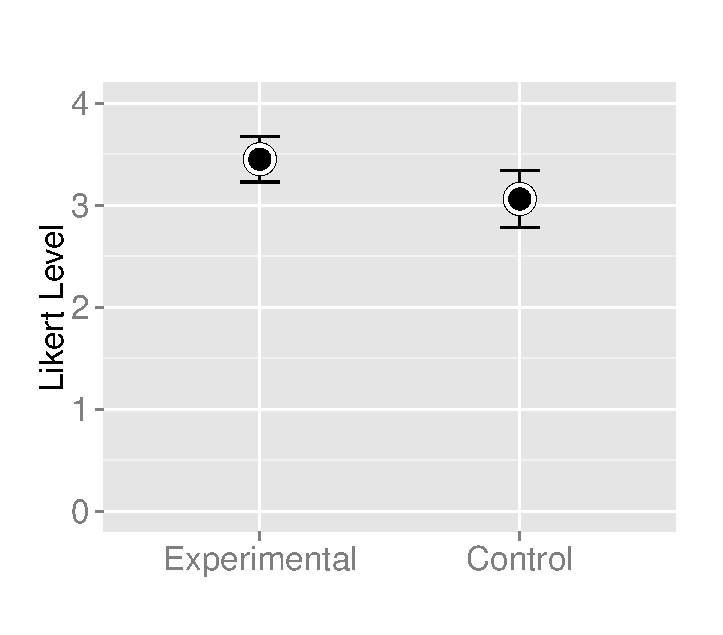
\includegraphics[scale=0.5]{img/contribution.eps}
		\caption{協調プログラミングにおけるフォロワの貢献}
		\label{fig:Contribution}
	\end{center}
\end{figure}


フォロワのアンケートの有効回答数は,53件(利用群20件,非利用群33件)であった.

「グループでプログラムを組むときに他のメンバーに対して遠慮しましたか」と尋ねたアンケートの結果を\figref{fig:Diffidence}に示す.図のエラーバーは95\%信頼区間を表す.利用群の平均は3.05(sd=0.80),非利用群の平均は2.55(sd=0.89)であった.t検定を行った結果,利用群と非利用群の平均の差は有意であった(両側検定:t(43.1)=2.08,p$<$.05).


「あなたはあなたのグループの作品作りに貢献できましたか」と尋ねたアンケートの結果を\figref{fig:Contribution}に示す.図のエラーバーは95\%信頼区間を表す.利用群の平均は3.45(sd=0.49),非利用群の平均は3.06(sd=0.81)であった.t検定を行った結果,利用群と非利用群の平均の差は有意であった(両側検定:t(50.1)=2.12,p$<$.05).


\begin{table}[tb] 
\caption{グループでのプログラミングの感想} 
\label{tab:free1}
\hbox to\hsize{\hfil
\begin{tabular}{c|p{7cm}}\hline\hline
S01	& いろんなアイディアが出てくるので、個人で作るよりも楽しく取り組めました。また、自分が分からないことを他のメンバの子が教えてくれたりしたのでよかったです。 \\\hline
S02	& 「○○をやりたい」という目的が同じでも、人によってやり方が違うのが面白いなと思った。\\\hline
S03	& グループ内での実力さが大きく、自分にできることを探すのに苦労しました。改めてすごいと思いました。このままではだめだと思い、本などを読んで改めて理解したいと思いました。 \\\hline
S04	& グループの中で一番プログラミングが苦手だと自負していたので、あまり貢献できていないような気がします。 \\\hline
S05	& メンバと予定が合わなくて大変だった。 \\\hline
S06	&  人の書いたコードを統合させる工程が非常に難しかった。\\\hline
\end{tabular}\hfil}
\end{table}


「グループでのプログラミングの感想の自由に記述してください」というアンケート項目の結果を\tabref{tab:free1}に示す.S01〜S03はポジティブな意見を抽出した.ポジティブな意見では,協力することで理解が進んだという旨の意見や,メンバ同士の議論からアイデアを創出できたという意見が見られた.S04〜S06はネガティブな意見を抽出した.ネガティブな意見では,能力差から貢献ができなかったという意見や,グループでのプログラミングの難しさについて書かれたものが見られた.


\begin{table}[tb] 
\caption{CheCoProについての感想} 
\label{tab:free2}
\hbox to\hsize{\hfil
\begin{tabular}{c|p{7cm}}\hline\hline
S07		& グループの人がどんなプログラミングをしているのか随時確認できて便利だと思った。 \\\hline
S08		& ファイルの受け渡しがとても楽で使いやすかったです。 \\\hline
S09		& 便利でありがたかったです!USBなどを使うよりも断然手間が省けました。 \\\hline
S10		& 同じ名前のファイルが上書きされることに気づかず上書きしてしまい少し困りました。 \\\hline
S11		& 一部だけファイルを取り込みたい。上書きしないようにしてもらいたい。 \\\hline
S12		&  思いのほかプログラムの共有が難しかった。\\\hline
\end{tabular}\hfil}
\end{table}


「CheCoProについての感想や追加してほしい機能などを自由に記述してください」というアンケート項目の結果を\tabref{tab:free2}に示す.S07〜S09はポジティブな意見を抽出した.ポジティブな意見では,メンバの編集を観察できることや取り込みの容易さに関する意見が見られた.S10〜S12はネガティブな意見を抽出した.ネガティブ意見では,全部取込の際に同名ファイルが上書きされる仕様の改善を求める意見が見られた.


%----------7.2--------
\section{インタラクションパターン}

CheCoProのログからインタラクション図を作成し,分析を行った結果,3つのインタラクションパターンが見られた.

\begin{figure}[tb]
	\begin{center}
		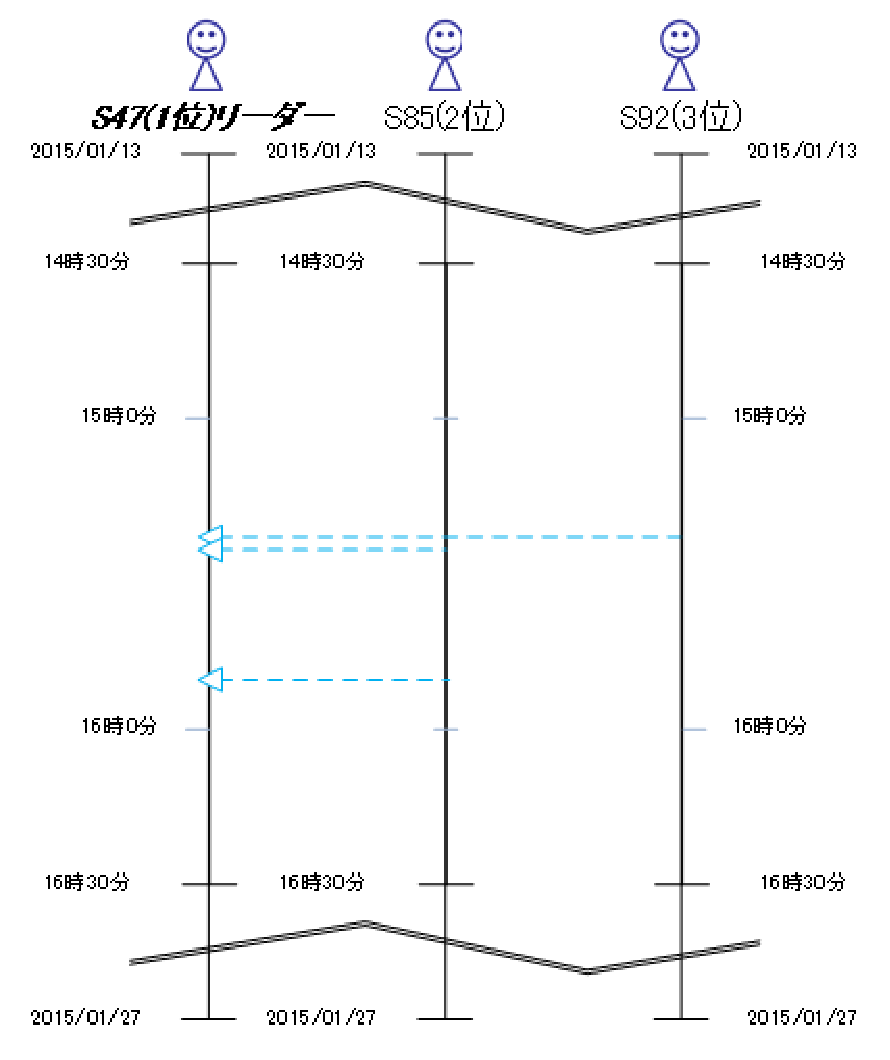
\includegraphics[scale=0.4]{img/flowK.eps}
		\caption{ソースコードの提供による貢献パターン(Group K)}
		\label{fig:flowK}
	\end{center}
\end{figure}

\begin{figure}[tb]
	\begin{center}
		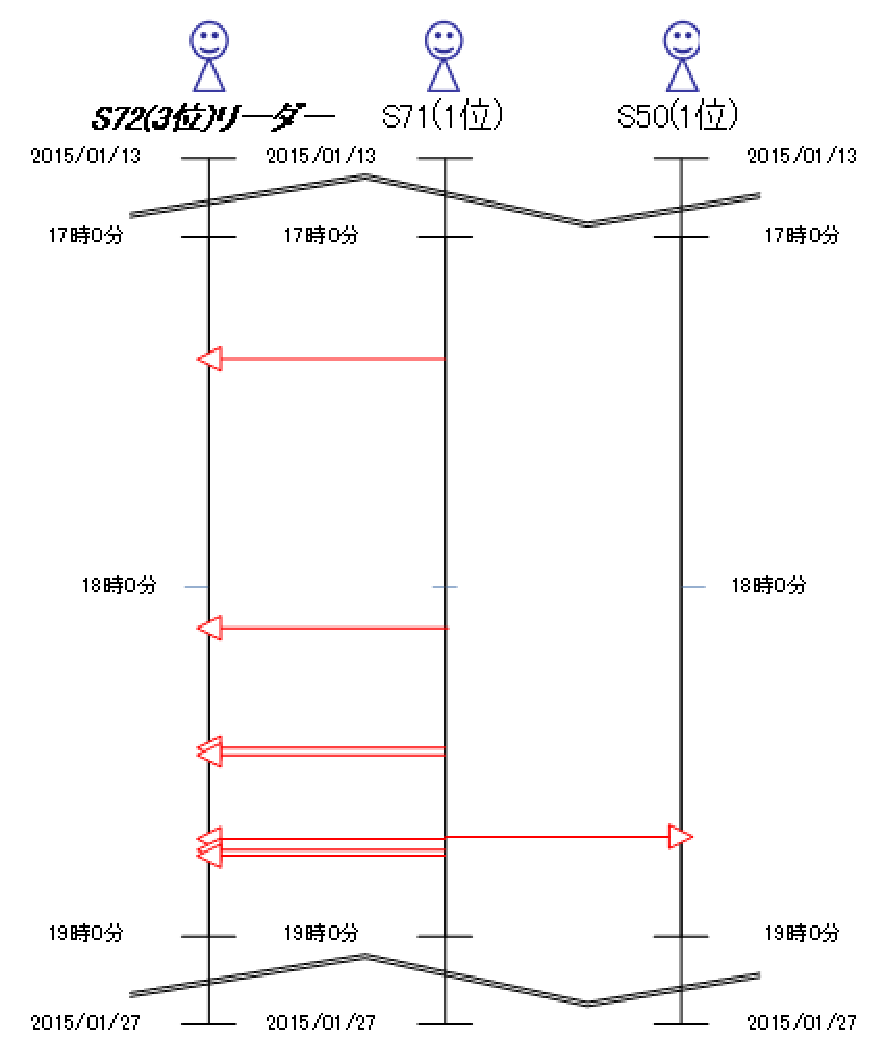
\includegraphics[scale=0.4]{img/flowL.eps}
		\caption{テストによる貢献パターン(Group L)}
		\label{fig:flowL}
	\end{center}
\end{figure}

\begin{figure}[tb]
	\begin{center}
		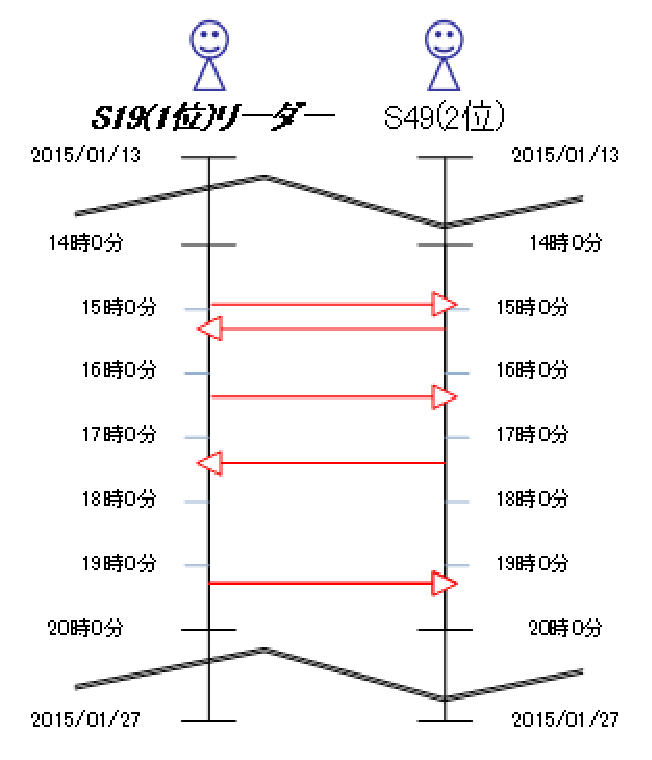
\includegraphics[scale=0.5]{img/flowE.eps}
		\caption{交互拡張(Group E)}
		\label{fig:flowE}
	\end{center}
\end{figure}

%----------7.2.1------
\subsection{ソースコードの提供による貢献}

フォロワが実装したプログラムの一部がドライバに取り込まれ,最終成果物の一部として採用されることがある.このパターンは全15グループ中7グループで見られた.

例としてグループKのインタラクション図の一部を\figref{fig:flowK}に示す.グループKのフォロワ(S85とS92)がドライバ(S47)のプロジェクトを全部取込していた.その後ドライバが各フォロワからプログラムの一部を取り込んでいる.

部分取込によって取り込まれたソースコードは,授業の教室を選ぶという,アドベンチャーゲームの1シーンである.S47はS85から別のシーンに関するソースコードも部分取込している.以上から,グループKのフォロワはそれぞれ担当するシーンについて責任を担い,実装をしていたと考えられる.


%----------7.2.2------
\subsection{テストによる貢献}

締め切り日の前夜にフォロワがドライバのプロジェクトを繰り返し全部取込するという現象が見られる.このパターンは全15グループ中6グループで見られた.

例としてグループLのインタラクション図の一部を\figref{fig:flowL}に示す.S72がS71から繰り返し全部取込をしていることから,フォロワがドライバのプログラムを繰り返しテストをするテスタとして貢献していると考えられる.ドライバのプログラムを何度も取り込んでいることから,テスト結果をドライバに報告し,ドライバがそれを基に修正をし,再びフォロワが全部取込を行ってテストをするというプロセスを繰り返している.

取り込み操作が容易なことから,変更が加わるたびに何度もテストを行うことに関して煩わしさが減少し,テストという観点でフォロワがプロジェクトに貢献しやすくなったと考えられる.


%----------7.2.3--------
\subsection{交互拡張}\label{Alternate extension}

グループメンバ同士で交互に全部取込をしている様子が見られる.このパターンは全15グループ中6グループで見られ,その全てが2人グループであった.

例としてグループEのインタラクション図の一部を\figref{fig:flowE}に示す.このパターンからは,ドライバとフォロワに関係なくお互いがプログラムを拡張していることが考えられる.グループEは,まずS49がS19の最新のものを取り込んでいる.取り込んだものを拡張して,拡張したものをS19が再度取り込んで拡張するということを繰り返してプロジェクトが進んでいると想定できる.


%----------7.3--------
\section{成績とインタラクション}


\begin{table}[tb]
	\caption{各グループメンバの成績} 
	\label{tab:records}
	\begin{tabular}{cc}
	\begin{minipage}{0.5\hsize}
  		\begin{center}
			\subcaption{グループL}\label{tab:groupL}
			\hbox to\hsize{\hfil
			\begin{tabular}{cc}\hline\hline
				ID		& 成績 \\\hline
				S72		& 51.5 \\
				S71		& 58.5 \\
				S50		& 58.5 \\\hline
			\end{tabular}\hfil}
		\end{center}
	\end{minipage}

	\begin{minipage}{0.5\hsize}
  		\begin{center}
			\subcaption{グループN}\label{tab:groupN}
			\hbox to\hsize{\hfil
			\begin{tabular}{cc}\hline\hline
				ID		& 成績 \\\hline
				S18		& 43.5 \\
				S30		& 54 \\
				S31		& 42.5 \\\hline
			\end{tabular}\hfil}
		\end{center}
	\end{minipage}
	\end{tabular}
\end{table}


\begin{figure}[tb]
	\begin{center}
		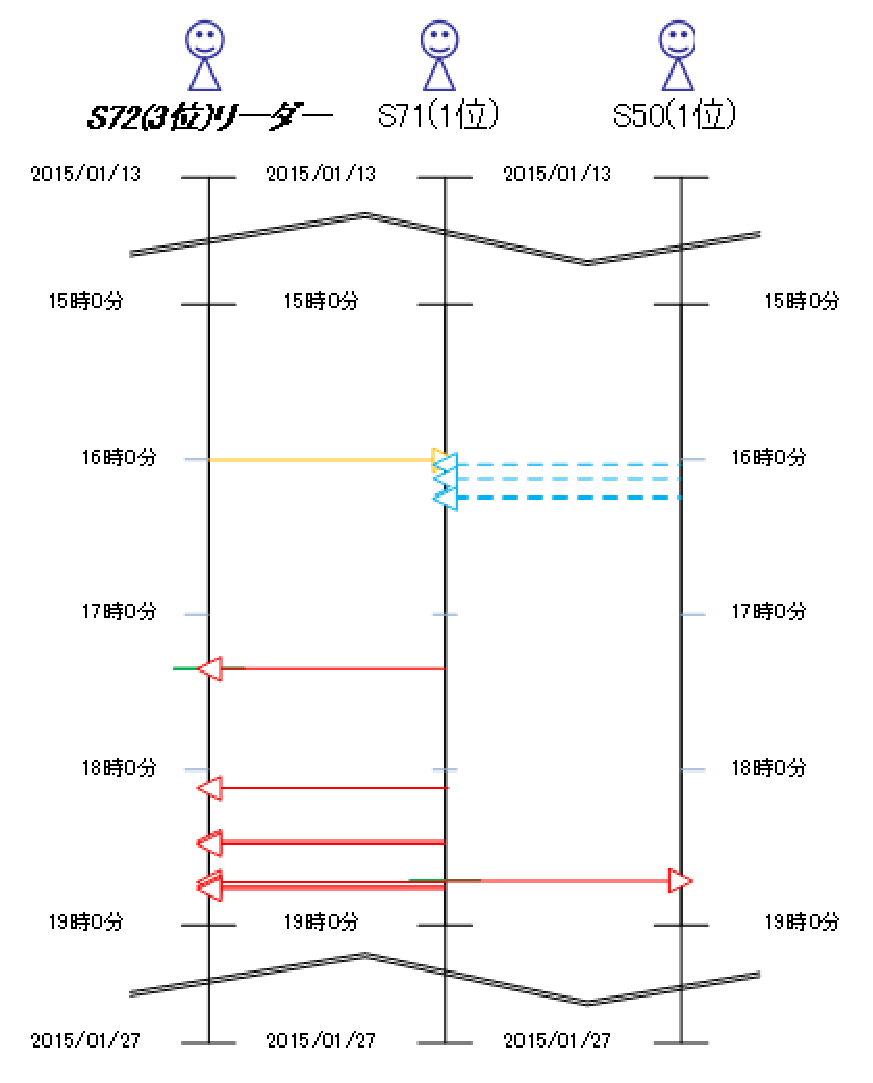
\includegraphics[scale=0.4]{img/flowL2.eps}
		\caption{グループLのインタラクション図}
		\label{fig:flowL2}
	\end{center}
\end{figure}


\begin{figure}[tb]
	\begin{center}
		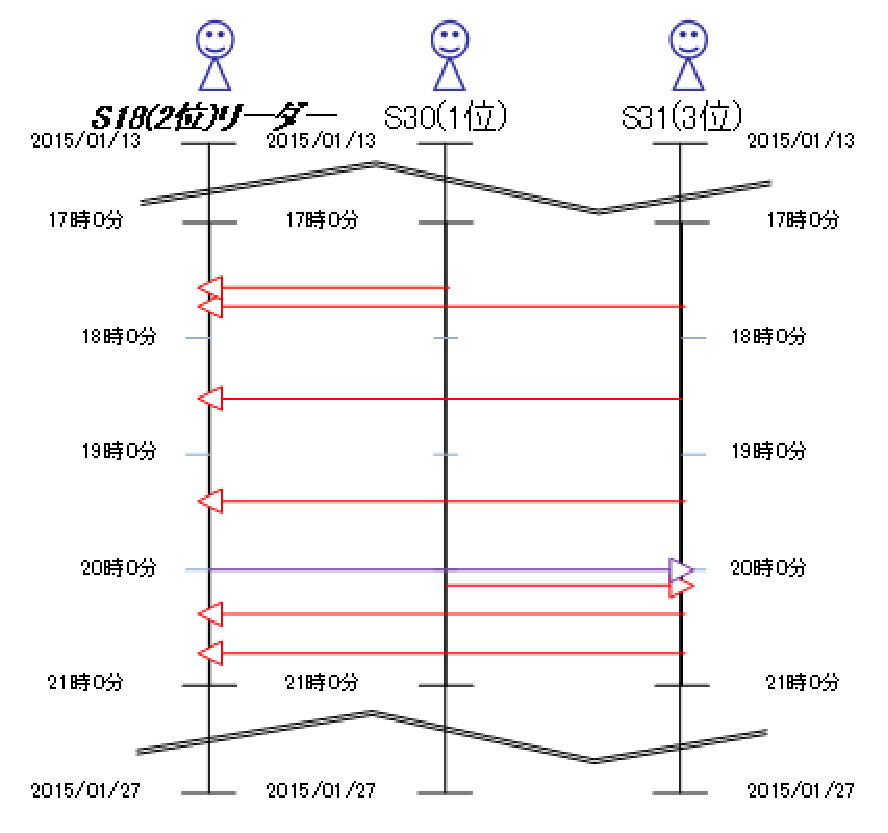
\includegraphics[scale=0.4]{img/flowN.eps}
		\caption{グループNのインタラクション図}
		\label{fig:flowN}
	\end{center}
\end{figure}


グループLのインタラクション図の一部を\figref{fig:flowL2},グループLの各メンバの成績を\tabref{tab:records}(a)に示す.S71は成績1位でドライバである.S50はドライバのS71ど同じ成績であり,ソースコードの一部で貢献している.S72は他のメンバと比べて成績が低く,テストで貢献している.

グループNのインタラクション図の一部を\figref{fig:flowN},グループNの各メンバの成績を\tabref{tab:records}(b)に示す.S30は成績トップでドライバである.S18はドライバのS30に比べて成績は低く,テストで貢献している.S31はS18と同等の成績でテストで貢献している.

以上のようなインタラクションから,各メンバが成績に見合った貢献ができていることがわかる.

\ref{Alternate extension}項で述べたように,交互拡張のパターンでは,各メンバが相手のソースコードを読んで拡張していることがわかる.しかし,グループN(\figref{fig:flowN})のように,成績差が大きいグループではソースコードの拡張までは行っていないメンバがいることがわかる.

\chapter{考察}\label{DC}

協調プログラミングの2つの要件(collective contributionとproductive interaction)の観点で考察を行う.2つの要件の達成度合いから本研究の限界を述べる.


\section{collective contribution}

成績に応じてソースコードの提供による貢献やテストによる貢献が行われていることから,各メンバが実力に見合った貢献ができていると考えられる.グループの2番手にあたるメンバはソースコードのレベルで貢献をし,3番手にあたるメンバはテストで貢献をしている.

プログラミングが苦手なメンバに対し,テストという点での貢献を促進できたことも1つの成果である.従来,3番手にあたるメンバは,プログラミングが苦手であるゆえに素材の作成を任されることが多かった.素材の作成による貢献もプロジェクトにおいて重要な作業である.テストもまた重要な作業である.テストにおいて,3番手にあたるメンバがプロジェクトに貢献する機会を用意することができた.

以上の成果は,独立同期モデルにおける取り込みの容易さに起因していると考えられる.全部取込と部分取込という2種類の取り込み方法を目的に応じて使い分けていることがわかった.


\section{productive interaction}

フォロワがドライバのソースコード編集の様子を観察していることや,積極的に取り込み操作が行われていることから,各メンバの能力が相乗的にプロジェクトに反映されている可能性がある.

観察とアンケートの自由記述からは,知識の伝播や創造的な議論が行われていることがわかった.

我々は,ソースコードに手をつけていないフォロワに,ドライバのソースコード編集の様子を観察・取り込みする機会を与えることができたことが大きな成果であると考える.非利用群においては,素材での貢献をするフォロワは,完成した素材をUSBメモリやメッセンジャーツール等でドライバに一方的に送るということが多く見られた.観察中に発見することはできなかったが,例えば画像のサイズがプログラムの動作にあっていない時に,フォロワが自らプログラムを書き換えて画像のサイズを調整するということも考えられる.このような知識創造の機会を与えることができた.

以上の成果は,独立同期モデルにおけるグループメンバの最新バージョンをリアルタイムに閲覧できることと,取り込みの容易さに起因していると考えられる.


\section{本研究の限界}

独立同期モデルが協調プログラミングの支援に一定の成果を挙げたが,いかなるグループに対しても有効に作用するわけではない.アンケートの自由記述において,グループでプログラムを組むことに対してネガティブな意見が見られた.典型的な例は,「プログラミングが苦手であるため貢献できなかった」という意見と,「個人で組むよりも気を遣ってしまい苦労をする」という意見である.

独立同期モデルが有効に働くか否かは,作品の内容,グループ内の能力差や各メンバの性格という様々な要因が重なることによって決まると考えられる.現状では,これらを測定する指標が曖昧なため,分析が困難である.例えば,プログラミング能力の指標として講義の成績を用いているが,成績がプログラミング能力に繋がるとは限らない.

支援可能なグループの幅を広げるために,協調プログラミングの実態をより明白にする必要がある.インタラクション図という形でファイルのやりとりを可視化したことで,初学者の協調プログラミングの実態を部分的に明らかにすることができた.協調プログラミング中のコミュニケーションなどのデータも取得し,インタラクション図と組み合わせたより詳細な分析が今後の課題である.

\chapter{結論}\label{CC}

プログラミング入門教育の場で,グループでプログラムを組む機会が設けられていることがある.初学者にとって協調プログラミングを行うことが困難となっている問題を解決するために,独立同期モデルを提案し,モデルに基づくシステムCheCoProを開発した.

CheCoProをプログラミング入門講義に導入し,協調プログラミングを実施した.CheCoProの利用ログとアンケートの結果を分析し,独立同期モデルの有効性の検証と協調プログラミングの実態解明を試みた.

その結果,協調プログラミングの2つの要件を充足すると解釈されるインタラクションパターンが見られた.アンケート結果も,グループメンバ間の能力差にかかわらず,個々のメンバが遠慮せず,より満足度の高い貢献を行うことができたことを示した.

\chapter*{謝辞}

本研究の全過程を通じてご指導頂きました静岡大学大学院情報学研究科の酒井三四郎教授,ならびに青山学院大学社会情報学部の松澤芳昭助教に深く感謝するとともに,厚く御礼申し上げます.また,本研究のに対するご指導・ご助言を頂きました,静岡大学情報学部の教員の皆様に御礼申し上げます.そして,研究の期間中,ご協力頂きました酒井研究室の皆様,ならびに実験にご協力頂きました情報学部の学生に心から感謝の意を申し上げます.

\newpage

\reference{reference}

\chapter*{著者発表論文}
\addcontentsline{toc}{chapter}{著者発表論文}
\begin{enumerate}
\renewcommand{\labelenumi}{[\arabic{enumi}]}

\item 静大花子, 情報太郎. 
プログラミング教育の研究.  
情報処理学会論文誌, vol.334, pp.334-352, 2014


\end{enumerate}

\end{document}